%--------------------------------------------------------------
\section{Análise de segurança}
%--------------------------------------------------------------
Para a análise de segurança das aplicações, cada qual publicada no \gls{heroku} e no \gls{vercel}, através de suas URLs próprias (ifriends-api e ifriends, respectivamente), foi feita uma análise pelo \href{https://www.ssllabs.com/}{SSL Labs}, visto que o \gls{heroku} utiliza um certificado básico com suporte para \acs{tls} 1.2 e \acs{hsts}, já que o suporte completo com o \acs{acme} na comunicação via \href{https://letsencrypt.org/getting-started/}{\textsl{Let's Encrypt}} e adição de certificados manuais, o \gls{heroku} só os disponibiliza \href{https://devcenter.heroku.com/articles/ssl}{ em versões pagas}. O \acs{vercel}, por outro lado, possui suporte completo para integração com o \acs{acme}, conforme descrito em sua \href{https://vercel.com/blog/automatic-ssl-with-vercel-lets-encrypt}{documentação oficial}.

De todo modo, é possível observar que ambas as aplicações receberam a nota mínima estipulada, conforme demonstrado na \autoref{analise_ssllabs_api_heroku} e na \autoref{analise_ssllabs_frontend_heroku}.

\begin{figure}[htb]
\centering
\caption{\label{analise_ssllabs_api_heroku} Análise de segurança na API}
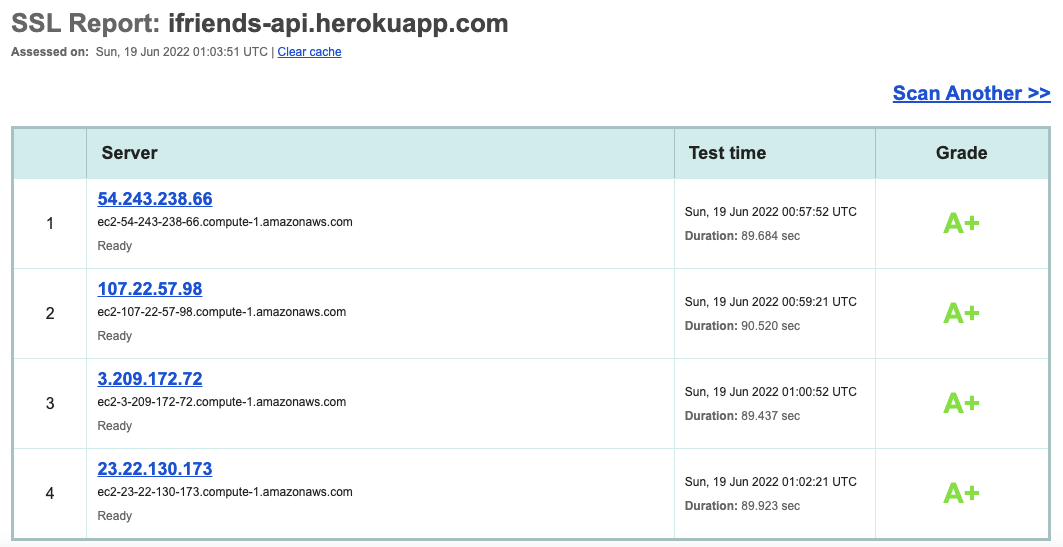
\includegraphics[width=1\textwidth]{anexos/Imagens_Seguranca/analise_ssllabs_api_heroku.png}
\fonte{Os autores}
\end{figure}
\FloatBarrier
A análise completa do que está descrito na \autoref{analise_ssllabs_api_heroku} também se encontra disponível para visualização em:  \href{https://www.ssllabs.com/ssltest/analyze.html?d=ifriends-api.herokuapp.com}{https://www.ssllabs.com/ssltest/analyze.html?d=ifriends-api.herokuapp.com}.

\begin{figure}[htb]
\centering
\caption{\label{analise_ssllabs_frontend_heroku} Análise de segurança no Front-end}
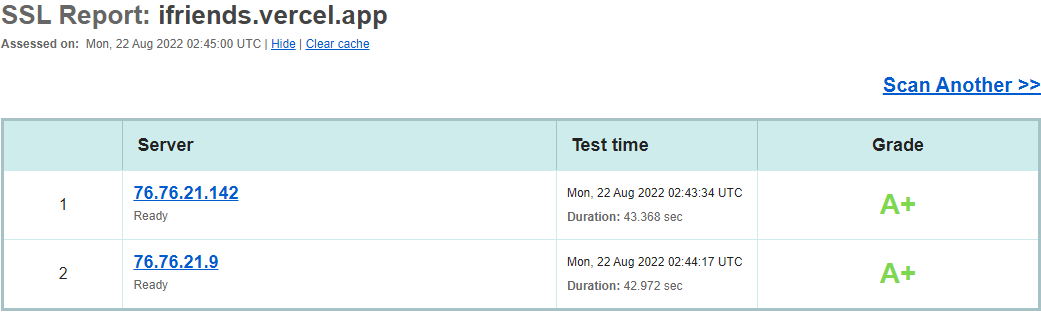
\includegraphics[width=1\textwidth]{anexos/Imagens_Seguranca/analise_ssllabs_frontend_heroku.png}
\fonte{Os autores}
\end{figure}
\FloatBarrier

A análise completa do que está descrito na  \autoref{analise_ssllabs_frontend_heroku} também se encontra disponível para visualização em:  \href{https://www.ssllabs.com/ssltest/analyze.html?d=ifriends.vercel.app}{https://www.ssllabs.com/ssltest/analyze.html?d=ifriends.vercel.app}.

Além disso, conforme os requisitos da disciplina, a \acs{api} teve suas respostas \acs{http} analisadas pelo \href{https://securityheaders.io}{\textit{Security Headers}}, e conforme observado na \autoref{analise_http_response_api}, a aplicação conseguiu configurar todos os cabeçalhos básicos de segurança requeridos na análise.

\begin{figure}[htb]
\centering
\caption{\label{analise_http_response_api} Análise de respostas HTTP na API}
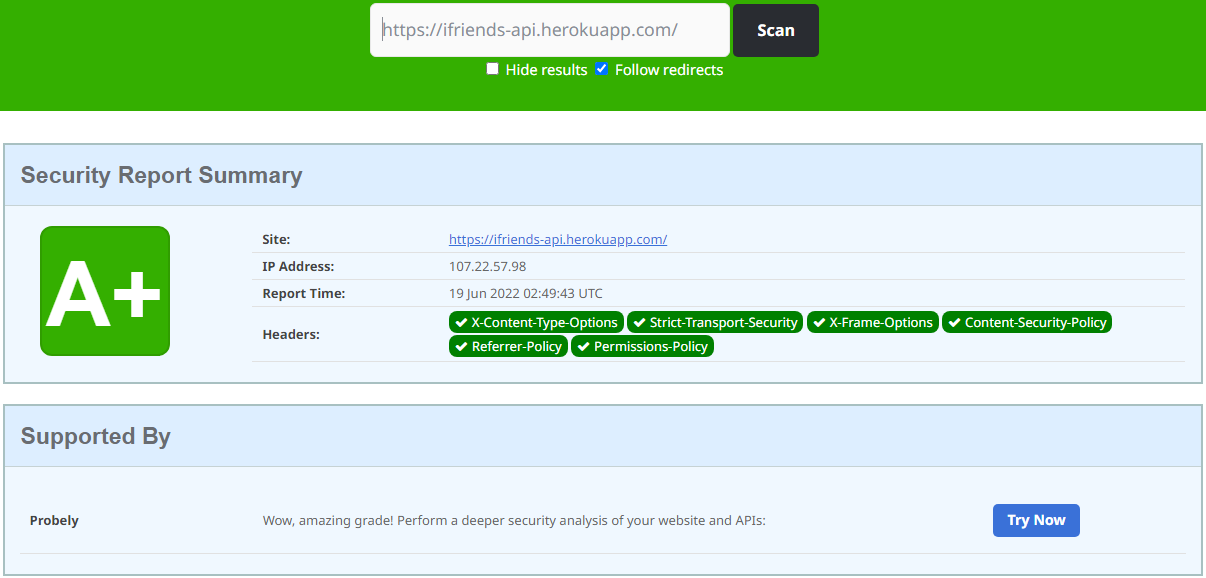
\includegraphics[width=1\textwidth]{anexos/Imagens_Seguranca/analise_http_response_api.png}
\fonte{Os autores}
\end{figure}
\FloatBarrier

Foi escolhido e aplicado pela equipe o \gls{vercel} como principal servidor de hospedagem para o lado do cliente, visto que ele possui todos os requisitos de segurança exigidos pela disciplina, assim como o certificado de \acs{dns} e suporte completo ao \acs{tls} de forma gratuita. Já para o servidor, sua hospedagem foi mantida no \gls{heroku} pela facilidade que ele oferece em hospedar o sistema juntamente com \acs{sgbd} já nativo do servidor, além de ser gratuito e ainda possuir barreiras mínimas de segurança.

\section{Análise estática de código}

De acordo com \citeonline{teixeira2007avaliaccao}, a análise estática tem como objetivo diminuir o impacto dos erros originados pelos próprios programadores sobre um determinado sistema/programa, conforme explica:

\begin{citacao}
As ferramentas de análise estática facilitam a detecção de anomalias ou erros de codificação existentes numa aplicação. Estas ferramentas vêm ajudar a eliminar lapsos cometidos
pelos programadores, podendo ter um impacto significativo no ciclo de desenvolvimento de
um produto, permitindo poupar tempo e dinheiro \cite{teixeira2007avaliaccao}.
\end{citacao}

Levando em conta os apontamentos feitos pelo autor, esta seção está reservada para algumas análises estáticas feitas sobre os códigos do \gls{ifriends} até o momento.

Foi utilizado o validador \textsl{FindBugs} como analisador estático do código feito em Java, isto é, da parte \gls{back-end} do sistema. O \textsl{FindBugs} possui uma integração amigável com o \gls{Eclipse}, facilitando a sua instalação no projeto \textsl{Spring Boot} desenvolvido atualmente. Além disso, o programa possui vários critérios de análise e classificações para os erros, deixando claros os riscos, caso passem despercebidos. A \autoref{relatorio analise estatica} mostra todos os pacotes e classes, assim como a quantidade de erros encontrados e outras informações sobre o projeto.

\begin{figure}[htb]
\centering
\caption{\label{relatorio analise estatica} Relatório do FindBugs}
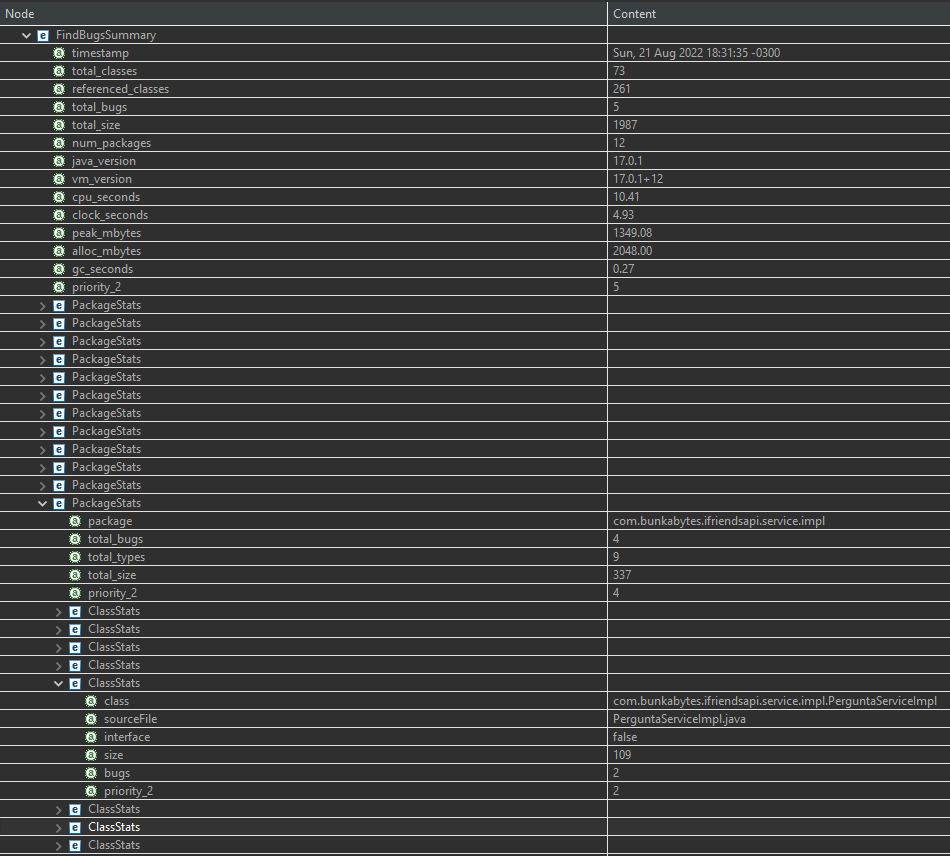
\includegraphics[width=1\textwidth]{anexos/Imagens_AnaliseEstatica/relatorio-findbugs.png}
\fonte{Os autores}
\end{figure}
\FloatBarrier

